% arara: pdflatex: { shell: yes }
\documentclass[twoside]{article}
\usepackage[utf8]{inputenc}
\usepackage[english]{babel}
\usepackage{amsmath, amssymb, amsthm}
\usepackage{hyperref}
\usepackage{ragged2e}
\usepackage{graphicx}
\usepackage{float}
\usepackage{fancyhdr}
\usepackage{geometry}
\usepackage{multicol}
\usepackage{url}
\usepackage{listings} % For better code formatting
\usepackage{xcolor} % For syntax highlighting

% Suppress underfull and overfull warnings
\tolerance=1000
\emergencystretch=10pt

\setlength{\headheight}{15.2pt}
\geometry{paperwidth=8.5in, paperheight=11.0in, top=1.0in, bottom=1.0in, left=1.0in, right=1.0in}

\pagestyle{fancyplain}
\fancyhead[LO]{Architecture of Blockchain Networks}
\fancyhead[CO]{}
\fancyhead[RO]{P25-LIS3122-1}
\fancyfoot[LO]{\thepage}
\fancyfoot[CO]{Networks and Telecommunications, UDLAP}
\fancyfoot[RO]{}

\begin{document}

\fancypagestyle{plain}{
  \renewcommand{\headrulewidth}{1pt}
  \renewcommand{\footrulewidth}{1pt}
}

\title{Architecture of Blockchain Networks}
\author{}
\date{\today}
\maketitle

\begin{abstract}
  \raggedright
  This document explores blockchain network architecture, focusing on decentralization, security, and scalability. It examines key components like consensus mechanisms, data structures, and interoperability solutions, while addressing challenges such as energy consumption and governance. Emerging innovations, including Layer-2 scaling and sharding, are highlighted to improve efficiency and scalability.
\end{abstract}

\begin{justify}
  \textbf{\textit{Keywords:}} architecture, blockchain, networks
\end{justify}

\section{Introduction}
Blockchain technology has emerged as one of the most transformative innovations of the 21st century, extending far beyond its initial application in cryptocurrencies. At its core, blockchain represents a novel approach to architecting data and coordinating network participants in a way that eliminates the need for trusted intermediaries \cite{reasearchgate}. This paradigm shift in network architecture has profound implications for various sectors, including finance, supply chain, healthcare, and governance.

The unique architecture of blockchain networks enables them to achieve seemingly contradictory goals: they are simultaneously decentralized yet coordinated, transparent yet secure, and immutable yet adaptable. Understanding how these networks are architected is essential for comprehending their capabilities, limitations, and potential applications. This paper aims to dissect the architecture of blockchain networks, examining both their internal components and external interactions.

By analyzing the architectural elements of blockchain systems, we can gain insights into how they achieve their core properties of decentralization, security, and transparency. Furthermore, this understanding can inform the design of more efficient and scalable blockchain networks, addressing current limitations in areas such as transaction throughput, energy consumption, and interoperability \cite{patnaik}.


\section{State of the art Study}
% need to add bitcoin and ethereum history reference
The architecture of blockchain networks has evolved significantly since the introduction of Bitcoin in 2009. Current blockchain architectures can be categorized based on various aspects, including access permissions, consensus mechanisms, and network topology.

\subsection{Network Topology and Node Types}
Blockchain networks typically follow a peer-to-peer (P2P) topology, where nodes connect directly without requiring central servers. However, the specific implementation varies across different blockchain systems. Bitcoin and Ethereum employ an unstructured P2P network where nodes connect randomly to each other, while other systems like Hyperledger Fabric use a more structured approach with defined roles for different node types \cite{patnaik}.

\begin{figure}[H]
  \centering
  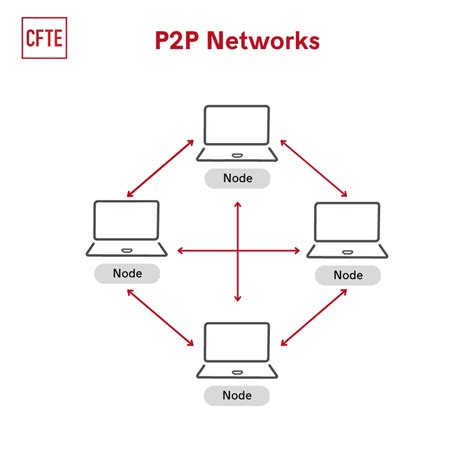
\includegraphics[width=1\textwidth]{imgs/p2p.jpeg}
  \caption{peer to peer network topology}
  \label{fig:1}
\end{figure}

Nodes in blockchain networks can serve various functions:
\begin{itemize}
  \item \textbf{Full nodes} maintain a complete copy of the blockchain and validate transactions and blocks.
  \item \textbf{Mining/Validator nodes} participate in the consensus process to add new blocks.
  \item \textbf{Light nodes} store only block headers and rely on full nodes for transaction verification.
  \item \textbf{Archive nodes} maintain the entire state history of the blockchain.
\end{itemize}

\subsection{Consensus Mechanisms}
Consensus mechanisms are critical components that enable distributed agreement on the state of the blockchain. Several approaches have emerged:

\begin{figure}[H]
  \centering
  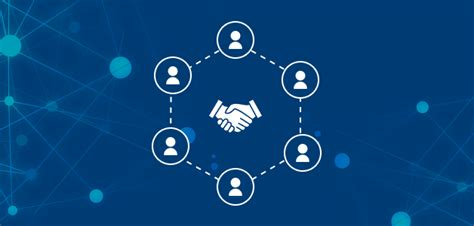
\includegraphics[width=1\textwidth]{imgs/conseuns.jpeg}
  \caption{Consensus mechanisms}
  \label{fig:2}
\end{figure}

\begin{itemize}
  \item \textbf{Proof of Work (PoW)}: Used by Bitcoin and (currently) Ethereum, requires nodes to solve computationally intensive puzzles.
  \item \textbf{Proof of Stake (PoS)}: Validators are selected based on the amount of cryptocurrency they hold and are willing to "stake" as collateral.
  \item \textbf{Delegated Proof of Stake (DPoS)}: Token holders vote for a limited number of delegates who validate transactions.
  \item \textbf{Practical Byzantine Fault Tolerance (PBFT)}: A voting-based consensus used in permissioned blockchains like Hyperledger Fabric.
  \item \textbf{Proof of Authority (PoA)}: Relies on a set of approved validators with known identities.
\end{itemize}

Each consensus mechanism presents different trade-offs between security, decentralization, and scalability \cite{reasearchgate}.

\subsection{Data Structures}
The fundamental data structure in blockchain is a linked list of blocks, where each block contains a set of transactions and a reference to the previous block (typically through a cryptographic hash). This creates an immutable chain where altering any block would require changing all subsequent blocks.

Beyond this basic structure, modern blockchains employ various data structures to enhance efficiency:
\begin{itemize}
  \item \textbf{Merkle Trees}: Enable efficient verification of transaction inclusion without downloading the entire block.
  \item \textbf{Patricia Tries}: Used in Ethereum to efficiently store and update state information.
  \item \textbf{Directed Acyclic Graphs (DAGs)}: Employed by systems like IOTA to allow for parallel transaction validation.
\end{itemize}

\subsection{Interoperability and Cross-Chain Communication}
As the blockchain ecosystem has expanded, the need for interoperability between different blockchain networks has become increasingly important. Projects like Polkadot, Cosmos, and Chainlink are developing protocols and infrastructure to enable secure cross-chain communication and asset transfers \cite{doi}. These interoperability solutions add another layer to blockchain network structures, creating a "network of networks" architecture.

\section{Analysis} 
The architecture of blockchain networks reveals several key insights about their functionality, limitations, and potential evolution.

\subsection{Architectural Enablers of Decentralization}
Decentralization in blockchain networks is achieved through a combination of architectural elements:

\textbf{Distributed Ledger}: By maintaining identical copies of the ledger across multiple nodes, blockchain eliminates single points of failure and control. This redundancy ensures that no single entity can unilaterally alter the transaction history \cite{patnaik}.

\textbf{Open Participation}: In public blockchains, the ability for anyone to operate a node without permission creates a diverse and geographically distributed network. This open architecture prevents geographic or jurisdictional centralization.

\textbf{Consensus Mechanisms}: By requiring agreement among a significant portion of network participants, consensus mechanisms distribute decision-making power. However, the specific implementation can significantly impact the degree of decentralization. For instance, PoW systems may lead to mining centralization due to economies of scale, while PoS systems might concentrate power among wealthy stakeholders \cite{reasearchgate}.

\subsection{Security Through Architecture}
The security of blockchain networks is intrinsically linked to their architecture:

\textbf{Cryptographic Linking}: The chained architecture of blocks, where each block references the previous one through cryptographic hashes, makes historical data tamper-evident. Altering a transaction would require changing all subsequent blocks, which becomes computationally infeasible as the chain grows.

\textbf{Economic Incentives}: The reward and penalty structures built into blockchain protocols align participants' interests with network security. In PoW systems, miners invest significant resources in hardware and electricity, creating a financial disincentive for malicious behavior.

\textbf{Network Redundancy}: The distributed nature of blockchain means that attacks must target multiple nodes simultaneously to be effective. This significantly raises the cost and complexity of attacks compared to centralized systems \cite{doi}.

\subsection{Architectural Challenges and Limitations}
Despite their innovative design, blockchain networks face several architectural challenges:

\textbf{Scalability Trilemma}: The current architecture of most blockchain networks forces trade-offs between decentralization, security, and scalability. Improving one dimension often comes at the expense of others.

\textbf{Energy Consumption}: The architecture of PoW consensus mechanisms necessitates significant energy expenditure, raising environmental concerns. While alternative consensus mechanisms like PoS substantially reduce energy requirements, they introduce different architectural challenges related to stake distribution and validator selection.

\textbf{Governance}: The decentralized architecture of blockchain networks complicates governance processes. Making protocol changes requires coordination among diverse stakeholders with potentially conflicting interests, which can lead to contentious forks and community divisions.

\subsection{Emerging Architectural Innovations}
To address these challenges, several structural innovations are emerging:

\textbf{Layer-2 Solutions}: These solutions build additional structural layers on top of existing blockchains to improve scalability. Examples include Lightning Network for Bitcoin and various rollup technologies for Ethereum.

\textbf{Sharding}: This approach horizontally partitions the blockchain, allowing different groups of validators to process different transactions simultaneously, potentially improving throughput without sacrificing decentralization.

\textbf{Cross-Chain Architectures}: Interoperability protocols are creating meta-structures that connect independent blockchains, enabling specialized chains to focus on specific use cases while maintaining the ability to communicate with other chains \cite{patnaik}.

\section{Conclusions}
The structure of blockchain networks represents a fundamental innovation in distributed systems design, enabling trustless coordination among participants without central authority. Through our analysis, several conclusions emerge:

First, the core structural elements of blockchain—distributed ledgers, cryptographic linking, and consensus mechanisms—work in concert to create systems with unique properties of decentralization, transparency, and immutability. These properties make blockchain particularly valuable for applications requiring trust minimization and censorship resistance.

Second, the specific structural choices in blockchain design involve inherent trade-offs. Different consensus mechanisms, network topologies, and data structures offer varying balances between security, scalability, and decentralization. There is no one-size-fits-all blockchain structure; rather, designs should be tailored to specific use case requirements.

Third, the evolution of blockchain structures is trending toward greater complexity and specialization. Multi-layer architectures, cross-chain communication protocols, and application-specific chains are emerging as solutions to the limitations of monolithic blockchain designs. This suggests a future blockchain ecosystem characterized by interconnected, specialized networks rather than a single dominant structure.

Fourth, governance architectures remain a critical challenge. The technical architecture of blockchain networks must be complemented by effective social coordination mechanisms to enable adaptation and evolution without compromising core principles.

Finally, as blockchain technology matures, its architectural design is increasingly influenced by regulatory considerations, industry standards, and user experience requirements. The purely technical focus of early blockchain designs is giving way to more holistic approaches that consider these broader contexts.

In conclusion, the architecture of blockchain networks continues to evolve, driven by the need to address current limitations while preserving the core benefits of decentralization and security. Understanding these architectural elements and their interactions is essential for developing more effective blockchain systems and for appropriately applying this technology to solve real-world problems \cite{reasearchgate, patnaik, doi}.

\begin{thebibliography}{9}
  \bibitem{doi}
  El-Rewini, Z., Sadatsharan, K., Selvaraj, D. F., Plathottam, S. J., \& Ranganathan, P. (2020). Cybersecurity challenges in vehicular communications. Vehicular Communications, 23(100214), 100214 from \url{https://doi.org/10.1016/j.vehcom.2019.100214}
  \bibitem{patnaik}
  Patnaik, M. (2023, December 8). Understanding the key components of blockchain network. AlmaBetter, from \url{https://www.almabetter.com/bytes/articles/components-of-blockchain}
  \bibitem{reasearchgate}
  (N.d.). Researchgate.net. Retrieved April 2, 2025, from \url{https://www.researchgate.net/publication/335501297_A_Brief_Essay_on_the_Blockchain}
\end{thebibliography}
\end{document}
